\documentclass[a4paper,fleqn]{cas-sc}

\usepackage[authoryear,longnamesfirst]{natbib}
\usepackage{xcolor}
\usepackage{seqsplit}

% Permite que tags longas do Ollama quebrem dentro da célula da tabela.
\newcommand{\ollamatag}[1]{\texttt{\seqsplit{#1}}}

% Per-column highlighting in result tables: best value in green, worst in red.
\newcommand{\melhor}[1]{\textcolor{green!55!black}{#1}}
\newcommand{\pior}[1]{\textcolor{red!80!black}{#1}}

\begin{document}
\let\WriteBookmarks\relax
\def\floatpagepagefraction{1}
\def\textpagefraction{.001}

\shorttitle{LLMs for AEC Standard Conversion to RASE}
\shortauthors{E. N. S. Brito et al.}

\title[mode=title]{A Comparative Analysis of Open-Source LLMs for Converting Architecture, Engineering and Construction Standards to the RASE Format}

\author[1]{Eike Natan Sousa Brito}
\cormark[1]
\ead{eike.sousa@hotmail.com}
\credit{Conceptualization, Methodology, Software, Writing - original draft}

\author[1]{Andr\'e Carvalho}
\ead{andre@dcomp.ufs.br}
\credit{Supervision, Writing - review \& editing}

\author[1]{Marco Ant\^onio Brasiel Sampaio}
\ead{marco.sampaio@ufs.br}
\credit{Supervision, Writing - review \& editing}

\affiliation[1]{organization={Universidade Federal de Sergipe},
            addressline={Cidade Universit\'aria Prof. Jos\'e Aloísio de Campos},
            city={S\~ao Crist\'ov\~ao},
            postcode={49100-000},
            state={Sergipe},
            country={Brazil}}

\cortext[1]{Corresponding author}

\begin{abstract}
The \textit{Building Information Modeling} (BIM) methodology organizes the planning and execution of construction projects around a detailed three-dimensional model, reducing rework and anticipating interferences before construction begins. This model, however, does not by itself solve the verification of design compliance against regulatory technical standards, whose interpretive nature makes automation an open problem. The RASE methodology (\textit{Requirement, Applicability, Selection, Exception}) addresses this gap by rewriting each normative excerpt as computable data, allowing BIM \textit{software} to verify compliance automatically; converting standards into this format, however, is still done manually, rule by rule, which becomes a bottleneck for automation. Natural Language Processing, and Large Language Models (LLMs) in particular, emerges as a promising path to automate this conversion, and can be adapted to the task through Prompt Engineering, a lightweight technique that adjusts only the instruction sent to the model. This dissertation comparatively evaluates six open-source LLMs (Llama, Dolphin, Gemma, Mistral, Alpaca, and Qwen) on the automatic conversion of Brazilian AEC technical standards to the RASE format, using Prompt Engineering exclusively across three successive normalization levels (N1: atomic segmentation of normative sentences; N2: RASE operator identification; N3: semantic JSON structuring). The comparison was carried out over five experiments (EN1, EN2, EN1N2, EN3, and EN1N2N3) on a dataset of 79 annotated NBR~9050 standards, with thirteen metrics across five families (lexical, semantic, distance-based, generation-oriented, and classification), with the models served locally through Ollama under an identical dataset, prompt, and hardware protocol. The results show that the three-level decomposition, relying solely on Prompt Engineering, is sufficient to produce valid RASE representations, reaching semantic similarity close to 0.90 in the best scenarios; Llama achieved the best overall average (0.730), leading the N3-level stages (EN3 and EN1N2N3), while Dolphin offered the best cost-benefit ratio, around ninety times faster in the chained pipeline.
\end{abstract}

\begin{keywords}
Machine Learning \sep Natural Language Processing \sep LLM \sep Prompt Engineering \sep BIM \sep RASE
\end{keywords}

\maketitle

%% ======================================================================
\section{Introduction}\label{sec:introduction}
Designing and reviewing civil engineering projects is a knowledge-intensive activity: it requires engineers to interpret regulations, reconcile heterogeneous information, and make decisions grounded in expertise accumulated over years of practice. Engineering Informatics studies how computational methods can support precisely these activities, turning the knowledge embedded in documents, models, and standards into a machine-processable form. Within this field, automating the verification of building designs against regulatory technical standards is a long-standing and still open problem, since these standards are written in natural language and demand interpretation. The present work can be characterized as a problem in this area: it uses Artificial Intelligence (AI) to convert technical standards into a computable representation that Building Information Modeling (BIM) tools can check automatically, a task that sits at the intersection of knowledge representation, Natural Language Processing, and engineering practice.

In Brazilian civil engineering, designing and inspecting works still involves a large amount of rework. Part of this waste stems from how projects are represented: 2D drawings, the sector's historical standard, hide clashes and omit information that only surfaces on the construction site. The move toward three-dimensional models and, more specifically, toward the \textit{Building Information Modeling} (BIM) methodology emerged as a response to this problem \citep{eastman2011}.

BIM organizes project planning and execution around a detailed 3D model. The methodology spans dimensions ranging from 3D to 7D: 3D for the geometric model itself; 4D for time scheduling; 5D for costs; 6D for sustainability; and 7D for post-construction operation management \citep{eastman2011}. BIM is not a piece of \textit{software} but a concept supported by computer systems such as CAD; it is implemented by tools such as Autodesk Revit and Graphisoft ArchiCAD.

Modeling in BIM makes it possible to visualize interferences before construction begins, reducing on-site rework. Typical applications range from design analysis to budgeting, including planning, modular coordination, and life-cycle management \citep{eastman2011}.

BIM, however, does not by itself solve the verification of designs against regulatory standards. Regulatory (or technical) standards are documents that establish mandatory requirements, criteria, and procedures to ensure the safety, quality, and performance of buildings; in Brazil, they are issued by the Brazilian Association of Technical Standards (ABNT) as NBRs, such as NBR~9050 on accessibility. Each jurisdiction maintains its own set of rules, generally written in natural language and interpretive in nature, which makes automated compliance checking an open problem \citep{dimyadi2013,solihin2015}.

Making these standards machine-checkable requires converting them into a computable representation. To this end, \citet{hjelseth2011} proposed the RASE methodology, which rewrites each normative excerpt as structured data decomposed into four attributes: \textbf{R}equirement (what must be met), \textbf{A}pplicability (where the rule applies), \textbf{S}election (options for complying with it), and \textbf{E}xception (cases in which the rule does not hold). Once organized in RASE, a standard enables tools integrated with BIM \textit{software}, such as Revit, to validate a design element by element \citep{santos2021}. The bottleneck lies upstream: converting a standard to RASE is still done manually, rule by rule, and because a BIM model may gather hundreds or thousands of elements subject to standards, the cost of this work grows quickly.

Automating this conversion requires recognizing patterns in natural-language text, a task for which Machine Learning (ML) is promising. The motivation is reinforced by BIM itself: the wider its adoption, the larger the volume of data generated by each project, attracting data scientists, professionals whose role is to turn large volumes of information into value for organizations \citep{davenport2012}. ML, a subfield of AI, studies how to build algorithms that learn patterns directly from data, without explicitly programming the rules \citep{tan2006}; from the learned patterns, these models make predictions and respond to novel situations. In civil engineering, AI already automates steps that once relied on human inspection, from detecting structural pathologies to forecasting construction schedules \citep{rane2023,liu2022}.

Three recent examples illustrate this movement. \citet{liu2022} combined BIM, ML, and design rules to optimize the construction assembly process, showing gains in efficiency and cost. \citet{alawadhi2023} trained Artificial Neural Networks on BIM data to recognize construction objects in photographs: synthetic images generated from the model produced effective semantic segmentation on real photographs, paving the way for the use of synthetic data in architectural problems. On another front, \citet{saka2024} fed a model with 2,280 demolition projects to predict waste circularity: the system estimates the amounts of recyclable material and routes waste to the appropriate landfill, supporting planning.

When the object of analysis is the normative text itself, automation falls to Natural Language Processing (NLP), a subfield of AI devoted to the computational treatment of human language in tasks such as translation, summarization, and text classification. Within NLP, Generative AI gathers the models capable of producing new content (text, image, or audio) from what they learned during training. Among its most relevant manifestations are Large Language Models (LLMs) \citep{zhao2023}, a category that includes OpenAI's ChatGPT \citep{openai2024} and Meta's Llama~3 \citep{llama3}.

LLMs are AI systems aimed at understanding and producing human language at scale. Training involves massive volumes of text, allowing the model to capture linguistic and contextual nuances. Almost all current LLMs use some variation of the \textit{transformer} architecture, chosen for its efficiency in processing long sequences \citep{zhao2023}.

Adapting these models to specific domains can follow different paths. The lightest and most accessible of them is Prompt Engineering (PE): instead of retraining weights or building a retrieval infrastructure, one adjusts only the instruction sent to the model.

In the AEC sector, LLMs can assist both in reading standards and in converting them into machine-processable formats \citep{fuchs2024}. Yet the literature still has gaps: one of them is precisely the interpretation of laws, codes, and regulatory standards, whose semantic complexity has historically challenged earlier AI methods \citep{fuchs2024}.

Faced with this gap, this work decomposes the conversion of standards to RASE into three successive normalization levels, supported solely by Prompt Engineering: level \textbf{N1} segments the normative sentence into atomic rules; \textbf{N2} identifies, in each rule, the RASE operators; and \textbf{N3} structures the result as JSON. Over this decomposition, six open-source LLMs (Llama, Dolphin, Gemma, Mistral, Alpaca, and Qwen) are compared, served locally, across five experiments that evaluate each level in isolation and in a chained pipeline. Output quality is assessed by nine textual-similarity metrics across four families: lexical (FuzzyWuzzy and TF-IDF), semantic (SBERT, BERTimbau, and Multilingual), distance-based (\textit{Word Mover's Distance} with FastText and NILC), and generation-oriented (BERTScore and ROUGE-L); these are complemented by four classification metrics (Accuracy, Precision, Recall, and F1-score).

The contributions of this work lie at the intersection of Architecture, Engineering and Construction (AEC) and Computing: for AEC, it applies NLP models to building-code checking and proposes successive normalization levels over the RASE methodology of \citet{hjelseth2011}; for Computing, it brings LLMs well established in the literature to a new domain and subjects them to a systematic performance evaluation.

\section{Background}\label{sec:background}

\subsection{Engineering Standards and the RASE Methodology}\label{sec:standards-rase}
Technical standards form the regulatory framework of the AEC sector: they define the minimum requirements of safety, performance, quality, and interoperability for designs. At the international level, the International Organization for Standardization (ISO) publishes standards adopted across many countries; in BIM, the consolidated reference is the ISO~19650 series, devoted to organizing and digitizing information about construction works \citep{iso19650}. Regardless of jurisdiction, each standard combines three textual layers: (i) definitions and references, with no direct verification value; (ii) prescriptive requirements, with numerical and geometric limits amenable to automated checking; and (iii) recommendations and exceptions, in free text, often conditioned on specific building categories. In all three layers the raw text is long, recursive, and heavily dependent on prior definitions, which makes the translation into computable rules a non-trivial and, today, predominantly manual task.

Applying these standards remains largely manual: the professional reads long passages, identifies the relevant requirements, and checks them item by item against the design. In a BIM model with hundreds or thousands of elements subject to simultaneous standards, this effort grows combinatorially; \citet{eastman2009} show that manual checking is costly, fragile, and hardly scalable, motivating research into automated rule-based checking. Automating it, however, faces three obstacles: the ambiguity and cross-references of the natural language in which standards are written \citep{dimyadi2013}; regional variation, which limits the reuse of what has already been formalized elsewhere \citep{dimyadi2013,solihin2015}; and the semantic difficulty of distinguishing, within a passage, what is a requirement, an applicability, and an exception, which calls for a standardized, tool-interoperable schema \citep{solihin2015}.

The response the literature has been consolidating is to structure the standard into a computable schema before verification. \citet{beach2015} demonstrate that a rule-based system automates regulatory compliance checking in construction once standards are formalized. Along these lines, \citet{hjelseth2015} proposed two complementary methodologies: Tx3 and RASE. Tx3 classifies each piece of regulatory information as \textbf{Transcribe} (instructions directly transcribable into computable rules), \textbf{Transform} (instructions that must be rewritten while preserving meaning), and \textbf{Transfer} (imprecise requirements that demand expert analysis). Transcribable and transformable elements are rewritten and submitted to RASE, which marks each normative passage with four logical operators \citep{hjelseth2011}: \textbf{R}equirement (the associated duty, usually expressed by the imperative ``must''), \textbf{A}pplicability (to whom or to what the requirement applies), \textbf{S}election (a subset of the applicability), and \textbf{E}xception (the cases excluded from the rule). Each operator further receives structured attributes such as object, property, comparator, value, and unit, bringing the text closer to a directly verifiable form. For instance, in the sentence ``the cross slope must be at most 2\% for indoor floors'', the applicability is ``floors'', the selection ``indoor'', and the requirement ``cross slope less than or equal to 2\%''. Once organized in RASE, a standard enables tools integrated with BIM \textit{software}, such as Revit, to validate a design element by element \citep{santos2021}. Applying RASE manually, however, reintroduces the very bottleneck it aims to remove: marking operator by operator requires an expert and does not scale to the volume of standards in the sector. At its core, identifying Requirement, Applicability, Selection, and Exception in a sentence is a text classification and structuring problem, exactly the kind of task that Machine Learning techniques learn from examples.

\subsection{Large Language Models and Textual Validation Metrics}\label{sec:llm-metrics}
Large Language Models (LLMs) are AI models that combine Machine Learning, deep neural networks, and Natural Language Processing techniques to understand and generate human language \citep{touvron2023}. They are typically pre-trained in an unsupervised fashion over billions of words, learning to predict sentence structure probabilistically, and adopt the \textit{Transformer} architecture \citep{vaswani2017}, efficient at handling contextual dependencies over long sequences. The release of ChatGPT and GPT-4 \citep{openai2024} popularized these models, and, as a response to closed models, open-weight alternatives such as LLaMA emerged \citep{touvron2023,llama3}. Among the techniques that specialize an LLM for a domain task without changing its weights, Prompt Engineering is the lightest: it consists of carefully designing the instruction sent to the model, an essential practice for obtaining context-appropriate responses \citep{brown2020}.

Evaluating an LLM's output in text-conversion tasks requires comparing it to a reference. Since exact matching is rarely desirable, because a correct paraphrase must also count as a hit, a set of similarity metrics is used, organized into four families \citep{jurafsky2009}. The \textbf{lexical} ones compare the surface form of the strings: FuzzyWuzzy, based on the Levenshtein distance, and cosine similarity over TF-IDF vectors \citep{manning2008}. The \textbf{semantic} ones rely on sentence embeddings that bring texts of equivalent meaning closer, such as Sentence-BERT \citep{reimers2019}, BERTimbau (specialized in Portuguese) \citep{souza2020}, and multilingual models. The \textbf{distance-based} ones measure the cost of aligning the word embeddings of one text to those of another, as in the Word Mover's Distance \citep{kusner2015}, runnable over FastText \citep{bojanowski2017} or NILC embeddings. The \textbf{generation-oriented} ones, originating in machine translation and summarization, measure how much the output reproduces the reference: BERTScore \citep{zhang2020bertscore}, which aligns tokens by contextual similarity, and ROUGE-L \citep{lin2004rouge}, based on the longest common subsequence. To these we add classification metrics (accuracy, precision, recall, and F1-score), derived from the confusion matrix, which make omissions and hallucinations explicit by treating evaluation as an information-extraction problem \citep{manning2008}.

\subsection{Related Work}\label{sec:related-work}
The integration of BIM with generative AI technologies is still little explored in the AEC sector, but it is the subject of a recent wave of work. \citet{rane2023} analyze the integration between BIM and models such as ChatGPT and Bard, identifying gains in design and decision-making, but pointing to persistent obstacles (lack of data standardization, security shortcomings, and the models' difficulty in interpreting the semantics of BIM data) and proposing an adoption framework. \citet{lin2023} present JULE, a chatbot that combines BIM and NLP to deliver real-time, on-site queries about component dimensions without opening the conventional interfaces, with high accuracy in intent recognition but conditioned on well-structured BIM data. \citet{sammou2024} apply GPT-3.5 and GPT-4 to 385 safety questions and three Prompt Engineering techniques (Prompt Direct, Chain-of-Thought, and Few-Shot): GPT-4 reached 84.6\% accuracy against 73.8\% for GPT-3.5, but both failed on emergency and calculation questions, exposing the fragility of technical reliability. Finally, \citet{samsami2024} show that generic prompts do not work in the AEC sector and that specific prompts reduce errors, although hallucinations in complex tasks and the need for external validation persist. Taken together, these works confirm the potential of LLMs in the sector but reveal a common gap: the absence of a structured, formal representation that translates normative content into computable rules. Without it, LLMs extract text and generate insights but do not convert the standard into something directly machine-verifiable, exactly the point this work addresses by coupling LLMs to the RASE methodology.

\section{RASE-PE: Converting Standards to RASE with Prompt Engineering}\label{sec:methodology}
The proposed methodology, here named \textbf{RASE-PE}, rests on three decisions: (i) decomposing the conversion of standards into the RASE format across three successive normalization levels (N1, N2, and N3); (ii) using Prompt Engineering as the sole model-specialization technique, without changing weights or building a retrieval infrastructure; and (iii) systematically comparing six open-source LLMs served locally through Ollama, under an identical dataset, prompt, and hardware protocol. The following subsections detail the three-level decomposition, the Prompt Engineering employed, the evaluated models, the dataset, the validation metrics, and, finally, the computational environment and the code structure.

\subsection{Three-Level Normalization}\label{sec:three-levels}
Moving from the raw text of a standard to the RASE representation in JSON requires three distinct reasoning steps: syntactic segmentation, semantic classification, and structured-attribute extraction. Asking for all of this in a single LLM call tends to degrade the output, with hallucinations, omissions, and invalid JSON. RASE-PE decomposes the task into three successive levels, isolating each decision and allowing each step to be validated separately:

\begin{itemize}
\item \textbf{N1: Atomic Segmentation.} Normative sentences often embed more than one coordinated rule (for example, ``the cross slope must be at most 2\% for indoor floors and at most 3\% for outdoor floors'' contains two rules). N1 breaks the original sentence into atomic items, with a single rule per item, a precondition for the next steps to correctly assign the RASE operators.
\item \textbf{N2: RASE Operator Identification.} From each atomic rule, N2 identifies which spans correspond to Requirement, Applicability, Selection, and Exception. It is the core of the formalization: without it, the text remains in natural language.
\item \textbf{N3: Semantic JSON Structuring.} Classifying a span as R, A, S, or E still leaves it in natural language; for automated checking against a BIM model, the data must be extracted into structured fields. N3 produces a JSON with the fields \textit{type}, \textit{object}, \textit{property}, \textit{comparation}, \textit{target}, and \textit{unit}.
\end{itemize}

The chaining N1~$\rightarrow$~N2~$\rightarrow$~N3 forms the complete RASE-PE \textit{pipeline} (Figure~\ref{img:pipeline}), from raw text to the structured RASE representation. To isolate the contribution of each level and measure error propagation along the chain, the evaluation is organized into five experiments, presented in Section~\ref{sec:results}.

\begin{figure}[ht]
\centering
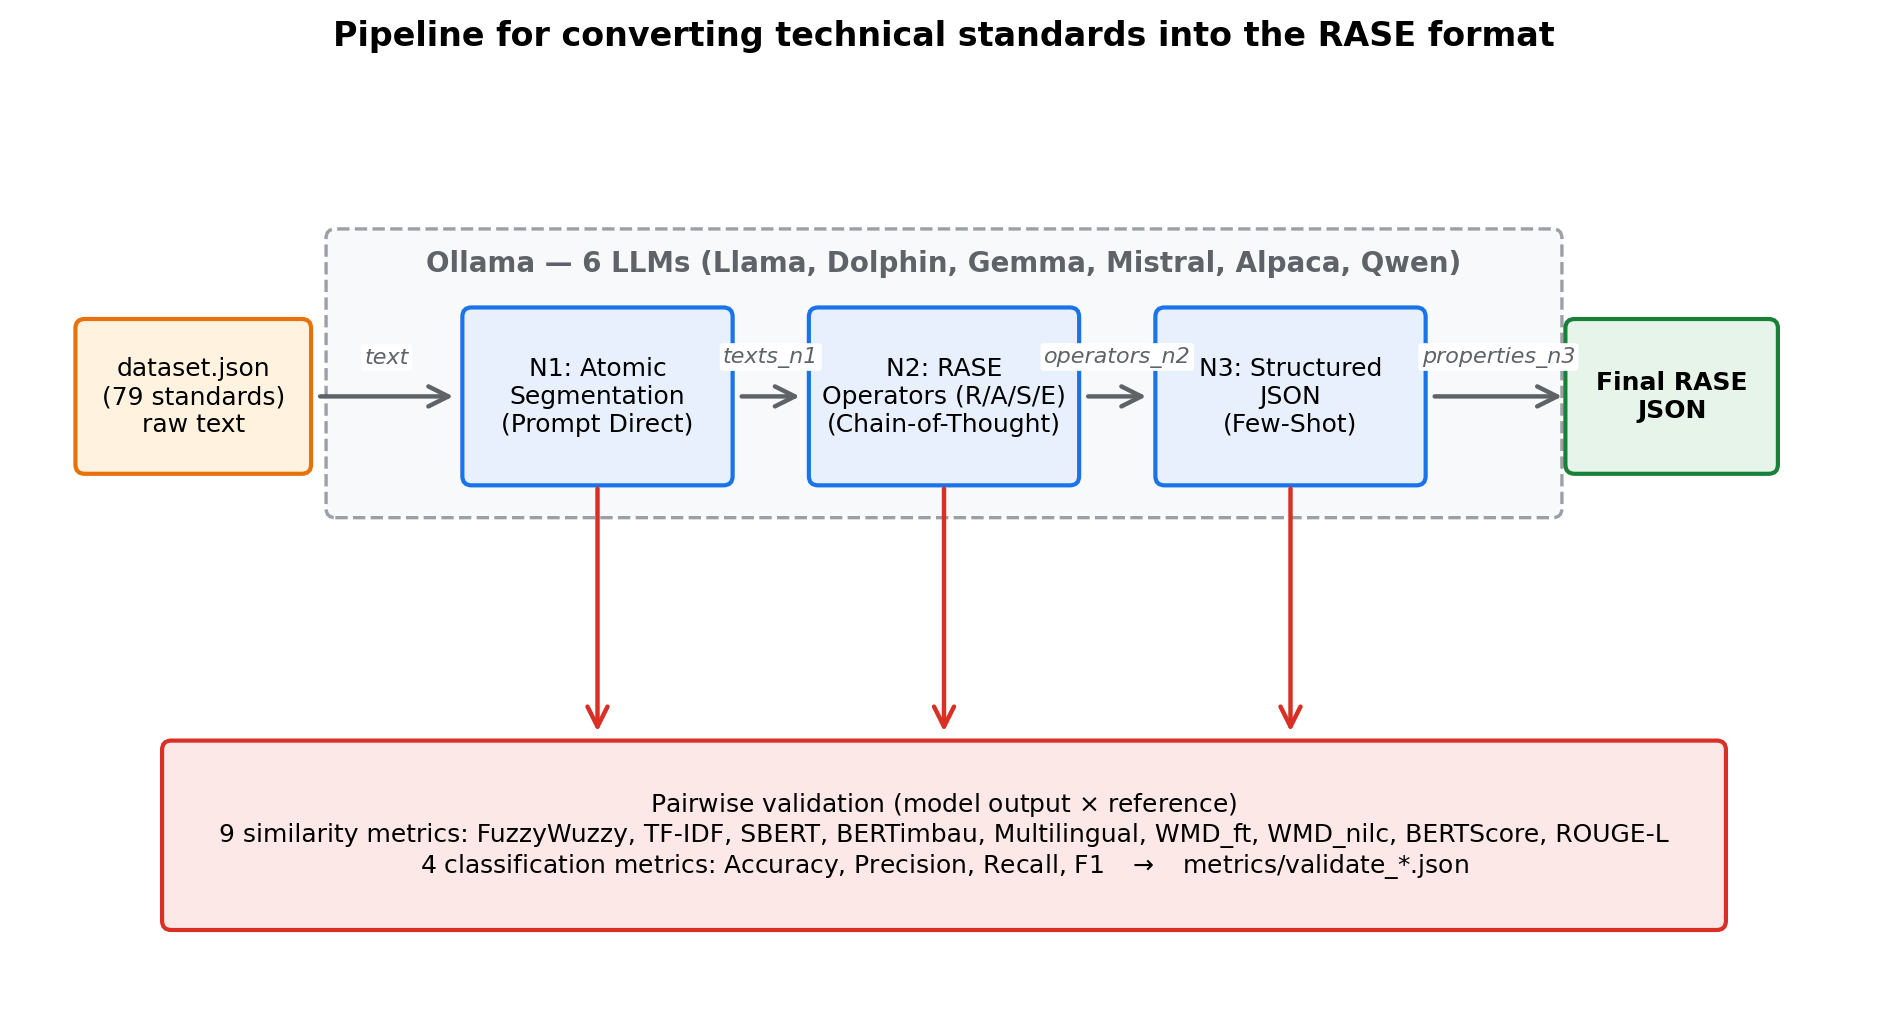
\includegraphics[width=0.98\linewidth]{figs/pipeline-en.png}
\caption{RASE-PE \textit{pipeline} for converting technical standards into the RASE format.}
\label{img:pipeline}
\end{figure}

\subsection{Prompt Engineering}\label{sec:prompt-engineering}
The specialization of the LLMs was carried out exclusively through Prompt Engineering: all task adaptation lives in the prompts, organized by level and by operator. Three classic techniques were applied, each chosen for the nature of the level it acts on. \textbf{N1} uses \textit{Prompt Direct}, a direct and objective instruction suited to a structurally simple task (segmenting the sentence into sub-rules) and economical in tokens and latency. \textbf{N2} uses \textit{Chain-of-Thought}, asking the model to make its reasoning explicit in steps before answering, which reduces hallucinations when classifying spans with multiple operators. \textbf{N3} uses \textit{Few-Shot}, embedding complete input--output examples that anchor the rigid JSON schema; since each RASE operator has a distinct nature, one prompt per operator was adopted (Applicability, Requirement, Selection, and Exception), each with the output schema, mapping heuristics based on common textual patterns (for example, ``public use'' $\rightarrow$ \textit{property} ``use'', \textit{comparation} ``='', \textit{target} ``public''), and its own examples.

\subsection{Evaluated LLMs}\label{sec:models}
Six open-source models were evaluated, run locally through Ollama \citep{ollama2024}, chosen for representing complementary profiles of size, alignment, language, and fine-tuning focus (Table~\ref{tab:models}). All share the decoder-only \textit{Transformer} architecture and the paradigm of massive pre-training followed by instruction post-training, but differ in data, alignment, and scale. Except for Llama, evaluated in its official general-purpose multilingual version, all were run from Brazilian-Portuguese-adapted checkpoints published by third parties and available in the Ollama registry. Running the six models on the same hardware, with the same prompts and the same dataset, is what ensures the comparability of the results.

\begin{table}[ht]
\centering
\caption{Evaluated open-source LLMs, with origin and the tag served through Ollama.}
\label{tab:models}
\footnotesize
\setlength{\tabcolsep}{4pt}
\begin{tabular}{@{}l l >{\raggedright\arraybackslash}p{5.3cm} l@{}}
\toprule
Model & Origin & Tag served through Ollama & Parameters \\
\midrule
Llama   & Meta                     & \ollamatag{llama3.1:8b}                                  & 8B \\
Dolphin & cnmoro (LLaMA-3 PT)      & \ollamatag{cnmoro/llama-3-8b-dolphin-portuguese-v0.3:4\_k\_m} & 8B (Q4\_K\_M) \\
Gemma   & brunoconterato (PT-BR)   & \ollamatag{brunoconterato/Gemma-3-Gaia-PT-BR-4b-it:f16}  & 4B (FP16) \\
Mistral & cnmoro (PT)              & \ollamatag{cnmoro/mistral\_7b\_portuguese:q4\_K\_M}      & 7B (Q4\_K\_M) \\
Alpaca  & splitpierre (Bode PT-BR) & \ollamatag{splitpierre/bode-alpaca-pt-br:13b-Q4\_0}      & 13B (Q4\_0) \\
Qwen    & cnmoro (PT)              & \ollamatag{cnmoro/Qwen2.5-0.5B-Portuguese-v1:q4\_k\_m}   & 0.5B (Q4\_K\_M) \\
\bottomrule
\end{tabular}
\end{table}

\subsection{Dataset}\label{sec:dataset}
The dataset was consolidated into a single JSON file with \textbf{79 annotated standards}, drawn from Brazilian AEC regulations, with emphasis on NBR~9050 \citep{abnt9050}, adapted from the work of \citet{eduardo2020}. NBR~9050 was chosen for its mostly prescriptive profile, with numerical values directly verifiable in a BIM model and well-delimited exceptions. Each entry gathers the reference RASE decomposition across the three levels: the raw text of the standard (\texttt{text}); the list of atomic rules (\texttt{texts\_n1}); for each rule, the four RASE operators (\texttt{operators\_n2}, with the keys \texttt{requeriments}, \texttt{aplicability}, \texttt{selection}, and \texttt{exception}); and, for each operator, the classified span (\texttt{text\_n2}) and the structured JSON properties (\texttt{properties\_n3}). Absent operators preserve the structure with empty strings. The same file serves both as input to the generators and as reference for the validators, simplifying reproducibility.

\subsection{Validation Metrics}\label{sec:metrics}
The evaluation combines thirteen metrics across five families. The nine \textbf{similarity} metrics (introduced in Section~\ref{sec:llm-metrics}) are computed pairwise between the predicted output and the reference, always on the normalized scale $[0,1]$: lexical similarity (FuzzyWuzzy and TF-IDF), semantic (SBERT-PT \texttt{tgsc/sentence-transformer-ult5-pt-small}, Legal-BERTimbau, and \texttt{paraphrase-multilingual-mpnet-base-v2}), distance-based (WMD over FastText and NILC embeddings), and generation-oriented (BERTScore and ROUGE-L). To these are added four \textbf{classification} metrics (accuracy, precision, recall, and F1-score), which treat the evaluation as information extraction and make omissions and hallucinations explicit. An element is \textit{positive} when filled and \textit{negative} when empty (\verb|""|); the matching criterion is semantic similarity above a threshold of 0.7 in N1 and N2, and exact equality (after normalizing case, accents, and punctuation) in N3. The 0.7 threshold balances rigor and tolerance to legitimate paraphrases; since it is applied equally to all models and experiments, it preserves the relative comparability among them.

\subsection{Computational Environment and Implementation}\label{sec:environment}
All runs were carried out on a single workstation (Intel Core i9-13900K CPU, 32~GB of RAM, NVIDIA RTX~4080 GPU, Ubuntu~22.04, Python~3.11), with the models served by Ollama (\texttt{ollama serve}) and the metrics computed with \texttt{sentence-transformers}, \texttt{gensim}, \texttt{fuzzywuzzy}, and \texttt{scikit-learn}. The pipeline was implemented as a modular Python project, orchestrated by a main script exposing three paths (data generation, validation, and table generation). The code is organized into packages by responsibility: \texttt{config/} (model registry and connection to Ollama), \texttt{prompts/} (the prompts as text files, one per level and one per operator in N3), \texttt{generates/} and \texttt{validates/} (one module per step, with a symmetric structure), \texttt{utils/} (auxiliary routines for cleaning, pairing, and metric computation), and the annotated \texttt{dataset.json}. This separation keeps each level isolated and makes the pipeline reproducible: switching models means only changing a configuration entry, and each experiment can be regenerated or revalidated independently. The complete source code is available at \url{https://github.com/EikESousA/Rase-PE}.

\section{Results and Discussion}\label{sec:results}

This section presents the results of applying the six open-source LLMs to the 79 Brazilian standards in the dataset, across the five experiments: EN1 (isolated N1 segmentation), EN2 (RASE identification with reference N1), EN1N2 (chained N1$\rightarrow$N2 pipeline), EN3 (JSON structuring in isolation, with reference N2), and EN1N2N3 (complete chained N1$\rightarrow$N2$\rightarrow$N3 pipeline). All figures come directly from the \textit{metrics/validate\_*.json} files, produced by the validation routine described in Section~\ref{sec:metrics}. For each experiment, the text reports the aggregate averages per metric, the detailed results per model, the execution times, and an integrated discussion.

\textbf{Table-reading convention.} In all numerical tables of this section, highlighting is done \textbf{per column}: the best value in each column appears in \melhor{green} and the worst in \pior{red}. In the quality tables (similarity and classification), values in \textbf{bold} are those within the similarity threshold adopted in validation, that is, \(\geq 0.7\) (Section~\ref{sec:metrics}). In the execution-time tables, where \emph{smaller is better}, \melhor{green} marks the fastest model and \pior{red} the slowest, and bold does not apply.

\subsection{Overview of the Experiments}

Table~\ref{tab:metricas_resultados} summarizes the per-metric averages across the five experiments, aggregated over the six models. Three patterns already stand out: embedding-based metrics (SBERT, BERTimbau, Multilingual, and BERTScore) keep consistently higher performance; the lexical ones (FuzzyWuzzy, TF-IDF, and ROUGE-L) lose ground as one moves from EN1 into EN1N2; and EN3 (isolated N3) rises to levels close to EN1 thanks to the restricted vocabulary of the JSON fields.

\begin{table}[ht]
\centering
\caption{Per-metric averages across the five experiments, aggregated over the six models.}
\label{tab:metricas_resultados}
\small
\begin{tabular}{lccccc}
\hline
Metric        & EN1   & EN2   & EN1N2 & EN3   & EN1N2N3 \\
\hline
\multicolumn{6}{@{}l}{\textit{Lexical similarity}} \\
\hspace{1em}FuzzyWuzzy & \pior{0.475} & 0.461 & 0.464 & \textbf{0.847} & 0.617 \\
\hspace{1em}TF-IDF & 0.636 & 0.312 & 0.417 & 0.597 & \pior{0.514} \\
\hline
\multicolumn{6}{@{}l}{\textit{Semantic similarity}} \\
\hspace{1em}SBERT & \textbf{0.801} & 0.490 & 0.594 & \melhor{\textbf{0.906}} & \textbf{0.777} \\
\hspace{1em}BERTimbau & \textbf{0.816} & 0.542 & 0.631 & \textbf{0.836} & \textbf{0.752} \\
\hspace{1em}Multilingual & \textbf{0.850} & 0.595 & 0.679 & \textbf{0.873} & \textbf{0.793} \\
\hline
\multicolumn{6}{@{}l}{\textit{Semantic distance (WMD)}} \\
\hspace{1em}WMD\_ft & \textbf{0.716} & 0.580 & 0.625 & \textbf{0.846} & \textbf{0.757} \\
\hspace{1em}WMD\_nilc & 0.688 & 0.546 & 0.595 & \textbf{0.842} & \textbf{0.742} \\
\hline
\multicolumn{6}{@{}l}{\textit{Generation-oriented metrics}} \\
\hspace{1em}BERTScore & \melhor{\textbf{0.866}} & \melhor{\textbf{0.753}} & \melhor{\textbf{0.790}} & \textbf{0.880} & \melhor{\textbf{0.843}} \\
\hspace{1em}ROUGE-L & 0.599 & 0.308 & \pior{0.404} & \textbf{0.765} & 0.616 \\
\hline
\multicolumn{6}{@{}l}{\textit{Classification metrics}} \\
\hspace{1em}Accuracy & \pior{0.475} & 0.273 & --- & 0.576 & --- \\
\hspace{1em}Precision & 0.545 & 0.202 & --- & \pior{0.024} & --- \\
\hspace{1em}Recall & \textbf{0.774} & 0.198 & --- & 0.380 & --- \\
\hspace{1em}F1-score & 0.631 & \pior{0.197} & --- & 0.043 & --- \\
\hline
\end{tabular}
\end{table}

The semantic metrics (SBERT, BERTimbau, and Multilingual), together with BERTScore, better preserved aggregate value across the five experiments, as they are more robust to surface variation. The lexical ones and ROUGE-L suffer from the rewording produced by the LLMs. In N3, the textual-similarity metrics rise to much higher levels than in N2 (quasi-structured, short output), but the exact-match classification metrics required in EN3 expose systematic difficulties: macro precision falls below 4\%. EN1N2N3 confirms the trend observed in EN1N2: the semantic metrics absorb error propagation well, while the lexical ones (TF-IDF and ROUGE-L) show a visible drop.

\subsection{Results per Experiment}

\subsubsection{EN1: N1 Segmentation}

In EN1, the comparison was between the N1 rules generated by the LLMs and the reference N1. The semantic metrics were well above the lexical ones (Multilingual~0.850, BERTimbau~0.816, and SBERT~0.801, against TF-IDF~0.636 and FuzzyWuzzy~0.475), indicating that segmentation tolerates lexical rewording when meaning is preserved. \textbf{Dolphin} dominated: it led in \textit{all} nine similarity metrics and in three of the four classification metrics, with the best individual performance of the experiment. The detailed figures are in Table~\ref{tab:resultados_en1}.

\begin{table}[ht]
\centering
\caption{Results per model in EN1 (similarity and classification).}
\label{tab:resultados_en1}
\scriptsize
\begin{tabular}{lccccccccc}
\hline
 & \multicolumn{2}{c}{Lexical} & \multicolumn{3}{c}{Semantic} & \multicolumn{2}{c}{WMD} & \multicolumn{2}{c}{Generation} \\
\cline{2-3}\cline{4-6}\cline{7-8}\cline{9-10}
Model & FW & TF-IDF & SBERT & BERTimbau & Multi. & WMD\_ft & WMD\_nilc & BERTScore & ROUGE-L \\
\hline
Alpaca  & 0.473 & 0.561 & \textbf{0.748} & \textbf{0.762} & \textbf{0.803} & 0.694 & 0.664 & \textbf{0.841} & 0.540 \\
Dolphin & \melhor{0.641} & \melhor{\textbf{0.756}} & \melhor{\textbf{0.873}} & \melhor{\textbf{0.891}} & \melhor{\textbf{0.913}} & \melhor{\textbf{0.774}} & \melhor{\textbf{0.751}} & \melhor{\textbf{0.905}} & \melhor{\textbf{0.703}} \\
Gemma   & 0.412 & 0.695 & \textbf{0.842} & \textbf{0.850} & \textbf{0.885} & \textbf{0.726} & 0.699 & \textbf{0.883} & 0.648 \\
Llama   & 0.422 & 0.672 & \textbf{0.835} & \textbf{0.844} & \textbf{0.873} & \textbf{0.711} & 0.684 & \textbf{0.871} & 0.605 \\
Mistral & 0.534 & \textbf{0.704} & \textbf{0.842} & \textbf{0.874} & \textbf{0.899} & \textbf{0.726} & 0.699 & \textbf{0.888} & 0.651 \\
Qwen    & \pior{0.367} & \pior{0.429} & \pior{0.668} & \pior{0.673} & \pior{\textbf{0.726}} & \pior{0.663} & \pior{0.632} & \pior{\textbf{0.808}} & \pior{0.448} \\
\hline
\multicolumn{10}{@{}l}{\textit{Classification metrics}} \\
Model   & \multicolumn{2}{c}{Accuracy} & \multicolumn{2}{c}{Precision} & \multicolumn{2}{c}{Recall} & \multicolumn{3}{c}{F1} \\
\hline
Alpaca  & \multicolumn{2}{c}{0.419} & \multicolumn{2}{c}{0.512} & \multicolumn{2}{c}{0.699} & \multicolumn{3}{c}{0.591} \\
Dolphin & \multicolumn{2}{c}{\melhor{0.676}} & \multicolumn{2}{c}{\melhor{\textbf{0.812}}} & \multicolumn{2}{c}{\textbf{0.801}} & \multicolumn{3}{c}{\melhor{\textbf{0.806}}} \\
Gemma   & \multicolumn{2}{c}{0.466} & \multicolumn{2}{c}{0.486} & \multicolumn{2}{c}{\melhor{\textbf{0.917}}} & \multicolumn{3}{c}{0.636} \\
Llama   & \multicolumn{2}{c}{0.446} & \multicolumn{2}{c}{0.479} & \multicolumn{2}{c}{\textbf{0.865}} & \multicolumn{3}{c}{0.616} \\
Mistral & \multicolumn{2}{c}{0.610} & \multicolumn{2}{c}{0.670} & \multicolumn{2}{c}{\textbf{0.872}} & \multicolumn{3}{c}{\textbf{0.758}} \\
Qwen    & \multicolumn{2}{c}{\pior{0.235}} & \multicolumn{2}{c}{\pior{0.311}} & \multicolumn{2}{c}{\pior{0.487}} & \multicolumn{3}{c}{\pior{0.380}} \\
\hline
\end{tabular}
\end{table}

Figure~\ref{img:4.2.1} presents the visual comparison among the six models across the nine similarity metrics in EN1.

\begin{figure}[ht]
\centering
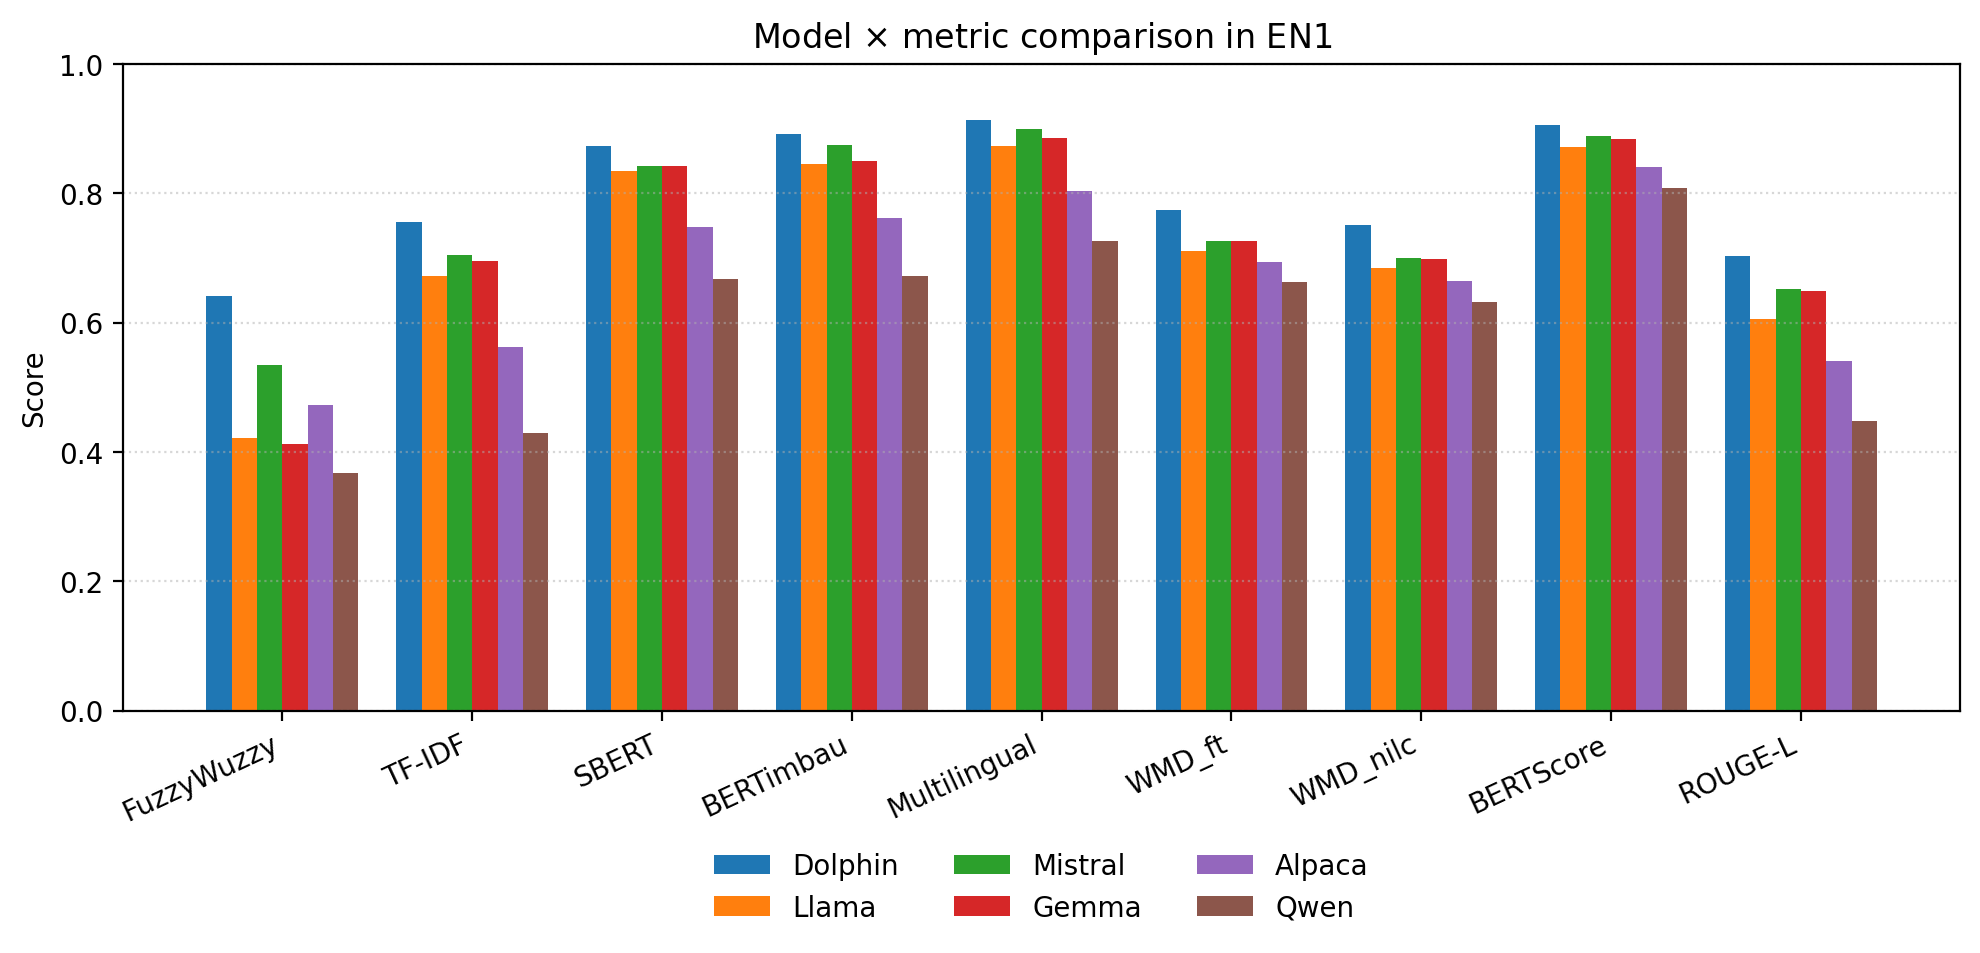
\includegraphics[width=0.95\linewidth]{figs/4.2.1-resultados-en1-barras-en.png}
\caption{Model $\times$ metric comparison in EN1.}
\label{img:4.2.1}
\end{figure}

\subsubsection{EN2: RASE Operator Identification}

EN2 measured the identification and structuring of the RASE operators from the reference N1. The averages dropped relative to EN1 (SBERT~0.490; Multilingual~0.595), reflecting the greater difficulty of structured formalization. The classification metrics fall even further (macro F1~0.197): the models have real difficulty distinguishing Selection and Exception. \textbf{Llama} leads in the semantic and lexical metrics; \textbf{Dolphin} takes the best macro F1 (0.286). The detailed figures are in Table~\ref{tab:resultados_en2}.

\begin{table}[ht]
\centering
\caption{Results per model in EN2 (similarity and per-operator macro classification).}
\label{tab:resultados_en2}
\scriptsize
\begin{tabular}{lccccccccc}
\hline
 & \multicolumn{2}{c}{Lexical} & \multicolumn{3}{c}{Semantic} & \multicolumn{2}{c}{WMD} & \multicolumn{2}{c}{Generation} \\
\cline{2-3}\cline{4-6}\cline{7-8}\cline{9-10}
Model & FW & TF-IDF & SBERT & BERTimbau & Multi. & WMD\_ft & WMD\_nilc & BERTScore & ROUGE-L \\
\hline
Alpaca  & \pior{0.334} & 0.168 & 0.386 & 0.418 & 0.484 & 0.522 & 0.486 & \textbf{0.702} & 0.172 \\
Dolphin & 0.511 & 0.423 & 0.557 & 0.621 & 0.665 & \melhor{0.620} & \melhor{0.589} & \textbf{0.786} & 0.412 \\
Gemma   & 0.384 & 0.364 & 0.520 & 0.579 & 0.625 & 0.608 & 0.577 & \textbf{0.772} & 0.350 \\
Llama   & \melhor{0.638} & \melhor{0.447} & \melhor{0.595} & \melhor{0.657} & \melhor{0.685} & 0.617 & 0.586 & \melhor{\textbf{0.796}} & \melhor{0.427} \\
Mistral & 0.563 & 0.385 & 0.575 & 0.607 & 0.665 & 0.607 & 0.575 & \textbf{0.779} & 0.377 \\
Qwen    & 0.336 & \pior{0.083} & \pior{0.304} & \pior{0.369} & \pior{0.444} & \pior{0.496} & \pior{0.462} & \pior{0.684} & \pior{0.111} \\
\hline
\multicolumn{10}{@{}l}{\textit{Classification metrics} (macro per operator)} \\
Model   & \multicolumn{2}{c}{Accuracy} & \multicolumn{2}{c}{Precision} & \multicolumn{2}{c}{Recall} & \multicolumn{3}{c}{F1} \\
\hline
Alpaca  & \multicolumn{2}{c}{\pior{0.081}} & \multicolumn{2}{c}{0.103} & \multicolumn{2}{c}{0.109} & \multicolumn{3}{c}{0.105} \\
Dolphin & \multicolumn{2}{c}{0.339} & \multicolumn{2}{c}{\melhor{0.301}} & \multicolumn{2}{c}{0.276} & \multicolumn{3}{c}{\melhor{0.286}} \\
Gemma   & \multicolumn{2}{c}{0.182} & \multicolumn{2}{c}{0.252} & \multicolumn{2}{c}{\melhor{0.300}} & \multicolumn{3}{c}{0.265} \\
Llama   & \multicolumn{2}{c}{\melhor{0.439}} & \multicolumn{2}{c}{0.237} & \multicolumn{2}{c}{0.250} & \multicolumn{3}{c}{0.243} \\
Mistral & \multicolumn{2}{c}{0.434} & \multicolumn{2}{c}{0.268} & \multicolumn{2}{c}{0.214} & \multicolumn{3}{c}{0.238} \\
Qwen    & \multicolumn{2}{c}{0.160} & \multicolumn{2}{c}{\pior{0.051}} & \multicolumn{2}{c}{\pior{0.039}} & \multicolumn{3}{c}{\pior{0.044}} \\
\hline
\end{tabular}
\end{table}

Figure~\ref{img:4.2.2} consolidates the performance of the six models across the nine similarity metrics in EN2.

\begin{figure}[ht]
\centering
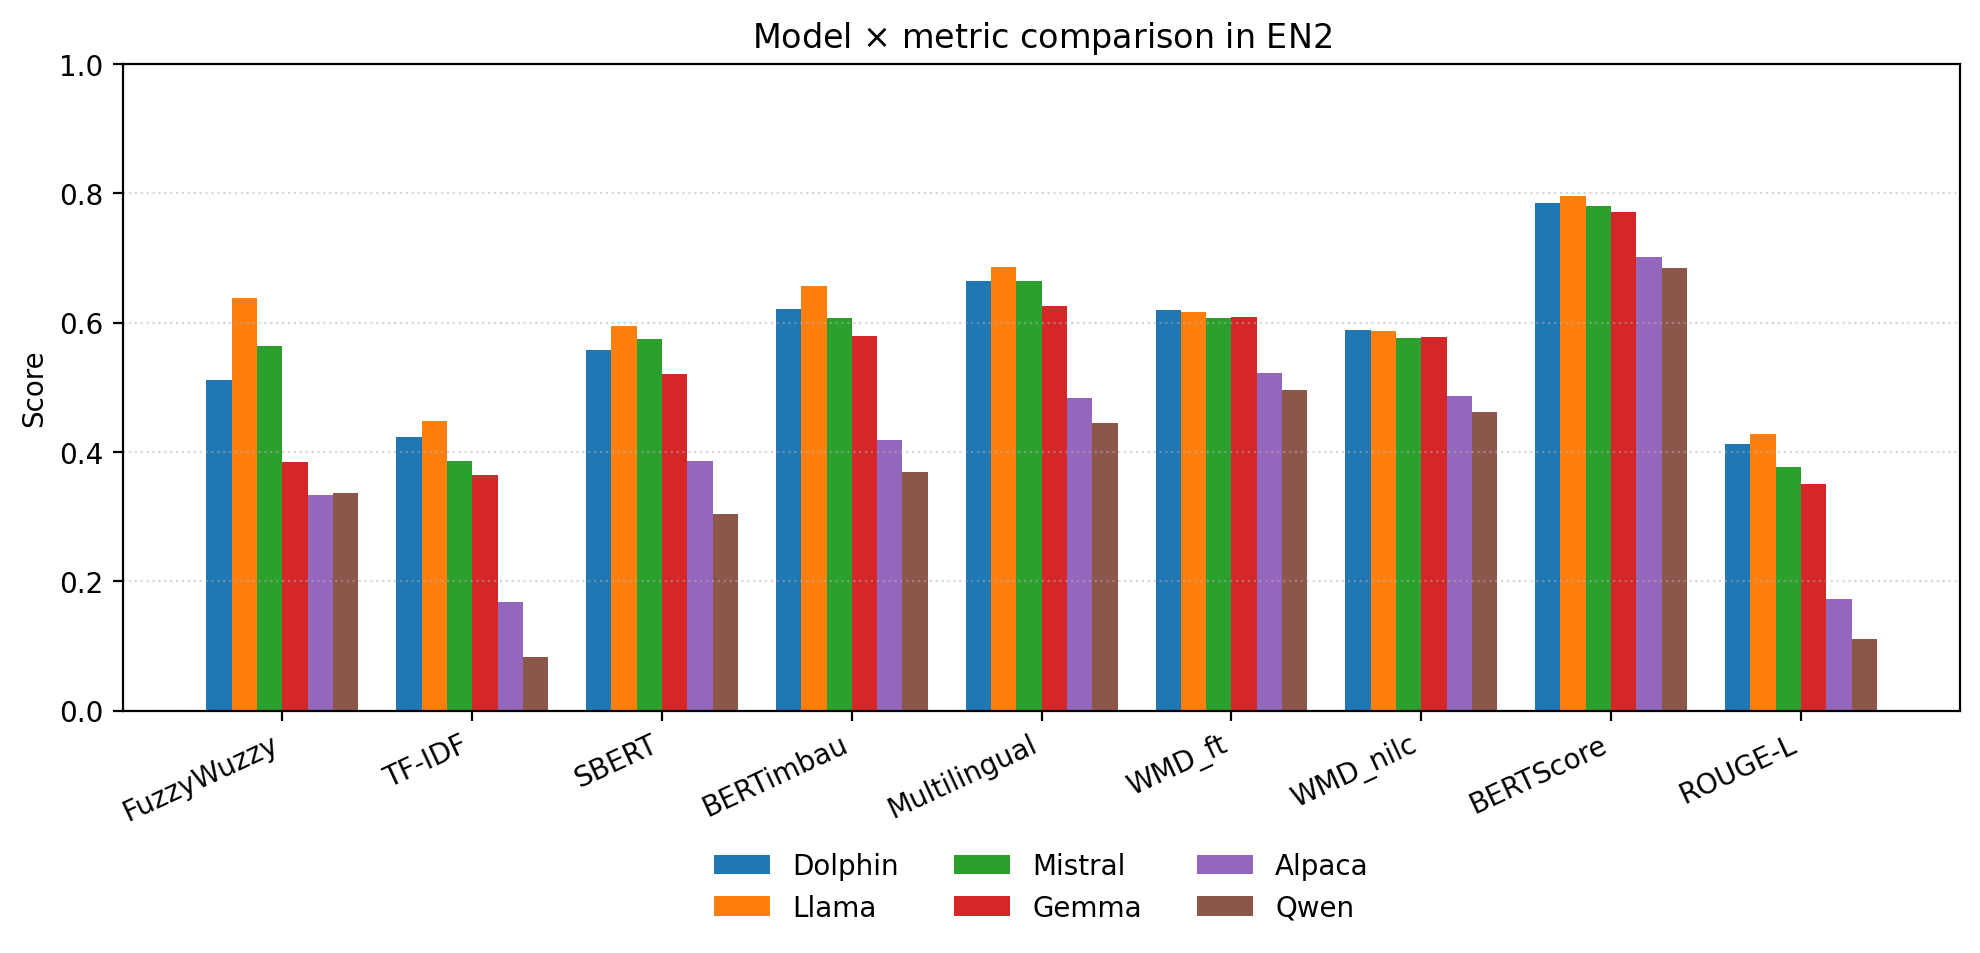
\includegraphics[width=0.95\linewidth]{figs/4.2.2-resultados-en2-barras-en.png}
\caption{Model $\times$ metric comparison in EN2.}
\label{img:4.2.2}
\end{figure}

\subsubsection{EN1N2: Chained Pipeline}

EN1N2 tested the robustness of the fully automated pipeline: the N1 produced by the model in the first stage feeds the N2 of the same model. The results confirm the \textbf{error-propagation} hypothesis, but with a surprise. The averages drop relative to EN2 in some metrics and stay close or even improve in others, as in the semantic ones: Multilingual rises from 0.595 to 0.679; BERTimbau from 0.542 to 0.631; SBERT from 0.490 to 0.594. The reason is that the pipeline produces outputs closer to the original sentences and, therefore, more aligned with the reference text at the semantic level, even though it loses precision in operator assignment. Leadership is shared: \textbf{Dolphin} dominates TF-IDF, WMD\_ft, WMD\_nilc, BERTScore, and ROUGE-L; \textbf{Llama} leads SBERT and ties in Multilingual. The full figures are in Table~\ref{tab:resultados_en1n2}.

\begin{table}[ht]
\centering
\caption{Results per model in EN1N2 (similarity).}
\label{tab:resultados_en1n2}
\scriptsize
\begin{tabular}{lccccccccc}
\hline
 & \multicolumn{2}{c}{Lexical} & \multicolumn{3}{c}{Semantic} & \multicolumn{2}{c}{WMD} & \multicolumn{2}{c}{Generation} \\
\cline{2-3}\cline{4-6}\cline{7-8}\cline{9-10}
Model & FW & TF-IDF & SBERT & BERTimbau & Multi. & WMD\_ft & WMD\_nilc & BERTScore & ROUGE-L \\
\hline
Alpaca  & 0.375 & 0.285 & 0.494 & 0.523 & 0.581 & 0.573 & 0.538 & \textbf{0.742} & 0.282 \\
Dolphin & 0.549 & \melhor{0.529} & 0.662 & \textbf{0.711} & \melhor{\textbf{0.749}} & \melhor{0.673} & \melhor{0.644} & \melhor{\textbf{0.826}} & \melhor{0.509} \\
Gemma   & 0.391 & 0.458 & 0.615 & 0.656 & \textbf{0.701} & 0.646 & 0.617 & \textbf{0.804} & 0.436 \\
Llama   & \melhor{0.570} & 0.521 & \melhor{0.677} & \melhor{\textbf{0.721}} & \melhor{\textbf{0.749}} & 0.649 & 0.620 & \textbf{0.821} & 0.488 \\
Mistral & 0.559 & 0.489 & 0.667 & 0.698 & \textbf{0.740} & 0.648 & 0.618 & \textbf{0.817} & 0.468 \\
Qwen    & \pior{0.342} & \pior{0.219} & \pior{0.448} & \pior{0.478} & \pior{0.551} & \pior{0.562} & \pior{0.530} & \pior{\textbf{0.731}} & \pior{0.240} \\
\hline
\end{tabular}
\end{table}

Figure~\ref{img:4.2.3} presents the visual comparison in EN1N2, highlighting the alternating leadership between Dolphin and Llama across metrics.

\begin{figure}[ht]
\centering
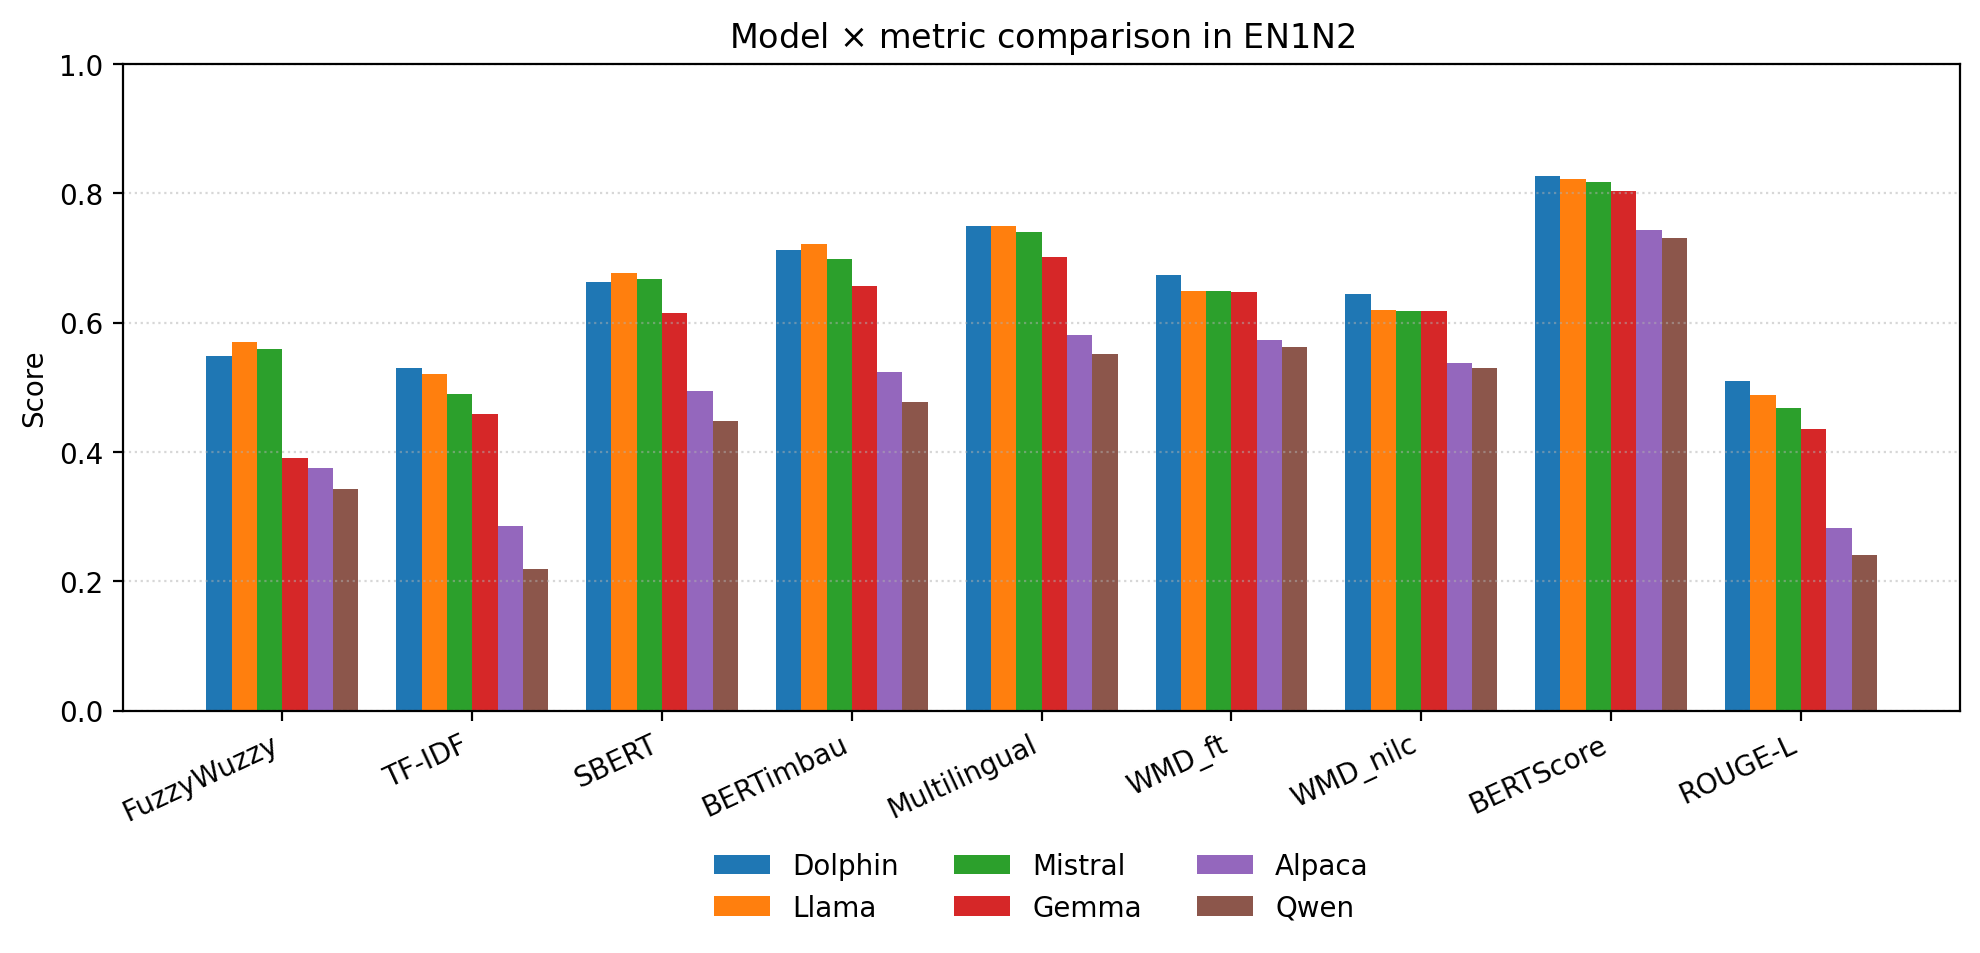
\includegraphics[width=0.95\linewidth]{figs/4.2.3-resultados-en1n2-barras-en.png}
\caption{Model $\times$ metric comparison in EN1N2.}
\label{img:4.2.3}
\end{figure}

\subsubsection{EN3: Semantic JSON Structuring with Reference N2}

Level N3 (semantic JSON structuring) was evaluated in two complementary scenarios: EN3, in isolation, taking the reference N2 operators as input; and EN1N2N3, in the end-to-end chained pipeline, in which the generated N1 feeds the N2 of the same model, which in turn feeds the N3 of the same model. In both scenarios, the comparison is not between whole normative strings, but field by field (\texttt{type}, \texttt{object}, \texttt{property}, \texttt{comparation}, \texttt{target}, and \texttt{unit}), over the canonical serialization of the generated JSON against the annotated JSON.

Since the output is \textit{quasi-structured} and made of short fields with restricted vocabulary, the textual-similarity metrics rise to much higher levels than in N1 and N2 (see Table~\ref{tab:resultados_n3}). The exact-match classification metrics, by contrast, paint a much harsher picture: macro precision falls below 4\%. This signals that the models preserve meaning but vary the vocabulary relative to the reference, for example \texttt{target = ``public''} instead of \texttt{target = ``public use''}. \textbf{Llama} dominated: it led in \textit{all} nine similarity metrics, with SBERT~0.947 and Multilingual~0.928. Mistral, Dolphin, and Qwen are close in the semantic metrics, showing that the isolated N3 stage is the most homogeneous among the evaluated models.

\begin{table}[ht]
\centering
\caption{Results per model in EN3 (similarity and per-field macro classification).}
\label{tab:resultados_n3}
\scriptsize
\begin{tabular}{lccccccccc}
\hline
 & \multicolumn{2}{c}{Lexical} & \multicolumn{3}{c}{Semantic} & \multicolumn{2}{c}{WMD} & \multicolumn{2}{c}{Generation} \\
\cline{2-3}\cline{4-6}\cline{7-8}\cline{9-10}
Model & FW & TF-IDF & SBERT & BERTimbau & Multi. & WMD\_ft & WMD\_nilc & BERTScore & ROUGE-L \\
\hline
Alpaca  & \pior{\textbf{0.729}} & \pior{0.395} & \pior{\textbf{0.846}} & \pior{\textbf{0.745}} & \pior{\textbf{0.798}} & \pior{\textbf{0.756}} & \pior{\textbf{0.751}} & \textbf{0.815} & \pior{0.624} \\
Dolphin & \textbf{0.860} & 0.694 & \textbf{0.912} & \textbf{0.848} & \textbf{0.887} & \textbf{0.842} & \textbf{0.839} & \textbf{0.901} & \textbf{0.799} \\
Gemma   & \textbf{0.751} & 0.480 & \textbf{0.858} & \textbf{0.755} & \textbf{0.823} & \textbf{0.762} & \textbf{0.757} & \pior{\textbf{0.810}} & 0.652 \\
Llama   & \melhor{\textbf{0.892}} & \melhor{\textbf{0.736}} & \melhor{\textbf{0.947}} & \melhor{\textbf{0.897}} & \melhor{\textbf{0.928}} & \melhor{\textbf{0.915}} & \melhor{\textbf{0.912}} & \melhor{\textbf{0.925}} & \melhor{\textbf{0.871}} \\
Mistral & \textbf{0.877} & 0.689 & \textbf{0.938} & \textbf{0.891} & \textbf{0.914} & \textbf{0.903} & \textbf{0.900} & \textbf{0.922} & \textbf{0.842} \\
Qwen    & \textbf{0.872} & 0.590 & \textbf{0.937} & \textbf{0.877} & \textbf{0.889} & \textbf{0.898} & \textbf{0.895} & \textbf{0.905} & \textbf{0.804} \\
\hline
\multicolumn{10}{@{}l}{\textit{Classification metrics} (macro per field)} \\
Model   & \multicolumn{2}{c}{Accuracy} & \multicolumn{2}{c}{Precision} & \multicolumn{2}{c}{Recall} & \multicolumn{3}{c}{F1} \\
\hline
Alpaca  & \multicolumn{2}{c}{\pior{0.283}} & \multicolumn{2}{c}{0.012} & \multicolumn{2}{c}{0.434} & \multicolumn{3}{c}{0.024} \\
Dolphin & \multicolumn{2}{c}{\textbf{0.705}} & \multicolumn{2}{c}{0.034} & \multicolumn{2}{c}{0.447} & \multicolumn{3}{c}{0.062} \\
Gemma   & \multicolumn{2}{c}{0.292} & \multicolumn{2}{c}{0.017} & \multicolumn{2}{c}{\melhor{0.603}} & \multicolumn{3}{c}{0.033} \\
Llama   & \multicolumn{2}{c}{\textbf{0.725}} & \multicolumn{2}{c}{\melhor{0.038}} & \multicolumn{2}{c}{0.361} & \multicolumn{3}{c}{\melhor{0.067}} \\
Mistral & \multicolumn{2}{c}{\melhor{\textbf{0.760}}} & \multicolumn{2}{c}{0.037} & \multicolumn{2}{c}{0.371} & \multicolumn{3}{c}{0.066} \\
Qwen    & \multicolumn{2}{c}{0.692} & \multicolumn{2}{c}{\pior{0.004}} & \multicolumn{2}{c}{\pior{0.063}} & \multicolumn{3}{c}{\pior{0.008}} \\
\hline
\end{tabular}
\end{table}

The setup was identical to that of the previous experiments: the same six LLMs served through Ollama, the same per-operator few-shot prompts, the same dataset of 79 standards. Per-model outputs are stored in dedicated JSON files (\texttt{generate\_n3\_<model>.json}); the aggregate lives in a single metrics file (\texttt{validate\_n3.json}). Exact per-field matching is harsher than the similarity threshold adopted in N1 and N2, which drives down the observed precision, especially in the models with weaker schema adherence (Alpaca and Qwen).

\subsubsection{EN1N2N3: Complete Chained Pipeline}

EN1N2N3 is the end-to-end automated pipeline. This is the scenario that replicates real production use: the sole input is the raw text of the standard, and the final output is the per-operator structured JSON. Since each stage accumulates transformations, it is also the experiment most subject to \textbf{error propagation}: the averages drop relative to isolated EN3 in all metrics (SBERT~0.777 \textit{vs.}~0.906; Multilingual~0.793 \textit{vs.}~0.873; BERTScore~0.843 \textit{vs.}~0.880). Even so, the absolute levels remain higher than those observed in EN2 and EN1N2, benefiting from the restricted JSON vocabulary. Table~\ref{tab:resultados_en1n2n3} reports the results per model.

\begin{table}[ht]
\centering
\caption{Results per model in EN1N2N3 (similarity over the structured JSON).}
\label{tab:resultados_en1n2n3}
\scriptsize
\begin{tabular}{lccccccccc}
\hline
 & \multicolumn{2}{c}{Lexical} & \multicolumn{3}{c}{Semantic} & \multicolumn{2}{c}{WMD} & \multicolumn{2}{c}{Generation} \\
\cline{2-3}\cline{4-6}\cline{7-8}\cline{9-10}
Model & FW & TF-IDF & SBERT & BERTimbau & Multi. & WMD\_ft & WMD\_nilc & BERTScore & ROUGE-L \\
\hline
Alpaca  & \pior{0.525} & \pior{0.345} & \pior{0.687} & \pior{0.645} & \pior{\textbf{0.701}} & \pior{0.676} & \pior{0.658} & \pior{\textbf{0.782}} & \pior{0.471} \\
Dolphin & 0.685 & 0.600 & \textbf{0.811} & \textbf{0.794} & \textbf{0.832} & \textbf{0.776} & \textbf{0.762} & \textbf{0.871} & 0.683 \\
Gemma   & 0.536 & 0.419 & \textbf{0.747} & \textbf{0.710} & \textbf{0.767} & \textbf{0.712} & 0.697 & \textbf{0.807} & 0.553 \\
Llama   & \melhor{\textbf{0.701}} & \melhor{0.630} & \melhor{\textbf{0.834}} & \melhor{\textbf{0.823}} & \melhor{\textbf{0.853}} & \melhor{\textbf{0.804}} & \melhor{\textbf{0.790}} & \melhor{\textbf{0.882}} & \melhor{\textbf{0.711}} \\
Mistral & 0.693 & 0.600 & \textbf{0.830} & \textbf{0.814} & \textbf{0.845} & \textbf{0.801} & \textbf{0.788} & \textbf{0.879} & 0.691 \\
Qwen    & 0.561 & 0.490 & \textbf{0.750} & \textbf{0.724} & \textbf{0.762} & \textbf{0.773} & \textbf{0.759} & \textbf{0.838} & 0.590 \\
\hline
\end{tabular}
\end{table}

Each model's output is persisted in its own JSON file (\textit{generate\_n1n2n3\_<model>.json}), and the aggregate metrics live in a single file (\textit{validate\_n1n2n3.json}). \textbf{Llama} keeps the lead it earned in isolated EN3, now across all nine similarity metrics; \textbf{Mistral} comes immediately behind, with marginal differences (Multilingual~0.845 \textit{vs.}~0.853). In line with the pattern observed in EN1N2, Llama, Mistral, and Dolphin retain their relative advantage in the full chain as well, whereas Alpaca and Gemma accumulate a drop across all metrics and deliver the worst overall performance, showing that failures in N1/N2 contaminate the final N3 structuring even in the semantic metrics.

\subsection{Results per Model}

Table~\ref{tab:ranking_global} reports the overall average per model, aggregating the nine textual-similarity metrics over the five experiments (EN1, EN2, EN1N2, EN3, and EN1N2N3). The final ranking departs from expectation: the leader is \textbf{Llama}, sustained by its absolute lead in EN3 and EN1N2N3 (both N3 stages) and by the best performance in EN2. \textbf{Dolphin} comes second: it dominates EN1 by a wide margin and keeps competitive performance in the following stages. Mistral comes third, followed by Gemma, Qwen, and Alpaca.

\begin{table}[ht]
\centering
\caption{Overall average per model (nine similarity metrics $\times$ five experiments).}
\label{tab:ranking_global}
\small
\begin{tabular}{lcccccc}
\hline
Model   & EN1   & EN2   & EN1N2 & EN3   & EN1N2N3 & Overall Avg. \\
\hline
Llama   & \textbf{0.724} & \melhor{0.605} & 0.646 & \melhor{\textbf{0.892}} & \melhor{\textbf{0.781}} & \melhor{\textbf{0.730}} \\
Dolphin & \melhor{\textbf{0.801}} & 0.576 & \melhor{0.650} & \textbf{0.843} & \textbf{0.757} & \textbf{0.725} \\
Mistral & \textbf{0.757} & 0.570 & 0.634 & \textbf{0.875} & \textbf{0.771} & \textbf{0.721} \\
Gemma   & \textbf{0.738} & 0.531 & 0.591 & \textbf{0.739} & 0.661 & 0.652 \\
Qwen    & \pior{0.602} & \pior{0.366} & \pior{0.456} & \textbf{0.852} & 0.694 & 0.594 \\
Alpaca  & 0.676 & 0.408 & 0.488 & \pior{\textbf{0.718}} & \pior{0.610} & \pior{0.580} \\
\hline
\end{tabular}
\end{table}

The per-model observations follow.

\textbf{Llama.} Leads the overall average (0.730) and dominates the N3-level experiments: in isolated EN3 it was ahead in \textit{all} nine metrics (SBERT~0.947; Multilingual~0.928; BERTScore~0.925); in EN1N2N3, it repeated the lead across the nine metrics (SBERT~0.834; Multilingual~0.853; BERTScore~0.882). It was also the best in EN2 in seven metrics: FuzzyWuzzy (0.638), TF-IDF (0.447), SBERT (0.595), BERTimbau (0.657), Multilingual (0.685), BERTScore (0.796), and ROUGE-L (0.427), in addition to the highest macro classification accuracy in the same experiment (0.439). In EN1N2, it led in FuzzyWuzzy (0.570), SBERT (0.677), and BERTimbau (0.721), tying with Dolphin in Multilingual (0.749). It is the choice when one can tolerate the computational cost.

\textbf{Dolphin.} It was the best segmenter in EN1, with absolute dominance in the nine metrics (BERTimbau~0.891; Multilingual~0.913; SBERT~0.873; BERTScore~0.905) and the best macro classification F1 in the experiment (0.806). In EN2, it led in WMD\_ft (0.620), WMD\_nilc (0.589), and macro F1 (0.286). In EN1N2, it was ahead in TF-IDF (0.529), WMD\_ft (0.673), WMD\_nilc (0.644), BERTScore (0.826), and ROUGE-L (0.509). In EN3 and EN1N2N3, it keeps competitive performance (SBERT~0.912 and 0.811, respectively), though behind Llama and Mistral. Added to this is its low computational cost (Section~\ref{sec:tempo}), which yields the best cost-benefit ratio observed.

\textbf{Mistral.} Consistent performance across all scenarios, and the most regular of the batch: third in the overall average (0.721), less than one percentage point behind the leader. It was close to the leaders in EN1 (Multilingual~0.899; BERTimbau~0.874) and in EN1N2 (Multilingual~0.740; BERTimbau~0.698), delivered the second-best macro accuracy in EN2 (0.434), and stays right next to Llama in EN3 (SBERT~0.938) and in EN1N2N3 (SBERT~0.830).

\textbf{Gemma.} Appears as the leader in macro classification recall in both EN1 (0.917) and EN2 (0.300), that is, good coverage with lower precision. Its semantic averages sit at an intermediate level.

\textbf{Alpaca.} Weak performance across all experiments, with a sharp drop in EN2 (SBERT~0.386; macro F1~0.105).

\textbf{Qwen.} Worst overall performance. It collapsed in EN2 (TF-IDF~0.083; macro F1~0.044) and had the highest latency in the chained pipeline (see Section~\ref{sec:tempo}). It is also weighed down by the model's tendency to generate outputs in simplified Chinese, outside the expected language.

\subsection{Analysis per Metric}

\textbf{Lexical metrics.} FuzzyWuzzy and TF-IDF drop clearly from EN1 to EN2 (FuzzyWuzzy: 0.475 $\rightarrow$ 0.461; TF-IDF: 0.636 $\rightarrow$ 0.312). Since they rely on lexical overlap, these metrics penalize the syntactic rewordings and synonymies generated by the LLMs. In EN3 and EN1N2N3, they rise again (FuzzyWuzzy: 0.847 and 0.617; TF-IDF: 0.597 and 0.514), benefiting from the short, restricted JSON vocabulary.

\textbf{Semantic metrics.} SBERT, BERTimbau, and Multilingual keep high and stable averages. BERTimbau, trained on Portuguese legal text, sits slightly above SBERT in almost every model and experiment (EN1: 0.816 \textit{vs.}~0.801; EN1N2: 0.631 \textit{vs.}~0.594), practical evidence of the gain from using domain embeddings to validate normative transformations. In EN3, they reach the highest values of the batch (SBERT~0.906; Multilingual~0.873), because the JSON fields contain short phrases with low lexical variation.

\textbf{Generation-oriented metrics.} BERTScore had the highest absolute average in EN2 (0.753) and in EN1N2 (0.790), thanks to the optimal alignment between tokens even under strong rewording. In EN3 and EN1N2N3, it stays high (0.880 and 0.843). ROUGE-L, in turn, behaved like a lexical metric, with a sharp drop in EN2 (0.308) and recovery in EN3 (0.765).

\textbf{Distance metrics (WMD).} Intermediate performance, between lexical and semantic. The values were highest in EN1 (WMD\_ft~0.716; WMD\_nilc~0.688) and in EN3 (WMD\_ft~0.846; WMD\_nilc~0.842), reflecting the greater lexical closeness between outputs and the reference text/JSON in those two scenarios.

\textbf{Classification metrics.} In EN1, macro F1 reaches 0.806 (Dolphin), indicating that most atomic sentences are segmented correctly. In EN2, F1 collapses to 0.286 in the best case (Dolphin), with a breakdown in Selection and Exception: F1 close to zero for all models. These two operators are especially hard to identify even for the leaders. In EN3, the low exact-match precision (macro precision below 4\% for all models) shows that token-by-token matching is too severe for a field whose semantics resists legitimate lexical variation.

\subsection{Execution Time}
\label{sec:tempo}

The total generation time was measured per model and per experiment. Table~\ref{tab:tempo_n1} reports the times in N1; Table~\ref{tab:tempo_n2}, in N2; Table~\ref{tab:tempo_n1n2}, in the chained N1N2 pipeline; Table~\ref{tab:tempo_n3} reports the EN3 times (isolated N3, with reference N2 as input); and Table~\ref{tab:tempo_n1n2n3}, those of the complete EN1N2N3 pipeline.

\begin{table}[ht]
\centering
\caption{Total generation time per model in N1.}
\label{tab:tempo_n1}
\begin{tabular}{lrr}
\hline
Model & Time (s) & Time (h:mm:ss) \\
\hline
Alpaca  & 104.55 & 0:01:44 \\
Dolphin & \melhor{62.65} & \melhor{0:01:02} \\
Gemma   & 133.04 & 0:02:13 \\
Llama   & \pior{5,676.97} & \pior{1:34:36} \\
Mistral & 70.04 & 0:01:10 \\
Qwen    & 309.59 & 0:05:09 \\
\hline
\end{tabular}
\end{table}

\begin{table}[ht]
\centering
\caption{Total generation time per model in N2.}
\label{tab:tempo_n2}
\begin{tabular}{lrr}
\hline
Model & Time (s) & Time (h:mm:ss) \\
\hline
Alpaca  & 249.10 & 0:04:09 \\
Dolphin & 124.69 & 0:02:04 \\
Gemma   & 244.19 & 0:04:04 \\
Llama   & \pior{6,895.71} & \pior{1:54:55} \\
Mistral & \melhor{123.63} & \melhor{0:02:03} \\
Qwen    & 6,515.09 & 1:48:35 \\
\hline
\end{tabular}
\end{table}

\begin{table}[ht]
\centering
\caption{Total generation time per model in N1N2.}
\label{tab:tempo_n1n2}
\begin{tabular}{lrr}
\hline
Model & Time (s) & Time (h:mm:ss) \\
\hline
Alpaca  & 330.84 & 0:05:30 \\
Dolphin & \melhor{104.28} & \melhor{0:01:44} \\
Gemma   & 427.22 & 0:07:07 \\
Llama   & 9,450.14 & 2:37:30 \\
Mistral & 138.39 & 0:02:18 \\
Qwen    & \pior{10,093.84} & \pior{2:48:13} \\
\hline
\end{tabular}
\end{table}

\begin{table}[ht]
\centering
\caption{Total generation time per model in N3 (isolated EN3).}
\label{tab:tempo_n3}
\begin{tabular}{lrr}
\hline
Model & Time (s) & Time (h:mm:ss) \\
\hline
Alpaca  & 2,104.92 & 0:35:05 \\
Dolphin & \melhor{584.96} & \melhor{0:09:45} \\
Gemma   & \pior{5,982.38} & \pior{1:39:42} \\
Llama   & 800.78 & 0:13:21 \\
Mistral & 627.68 & 0:10:28 \\
Qwen    & 847.41 & 0:14:07 \\
\hline
\end{tabular}
\end{table}

\begin{table}[ht]
\centering
\caption{Total generation time per model in N1N2N3 (complete pipeline).}
\label{tab:tempo_n1n2n3}
\begin{tabular}{lrr}
\hline
Model & Time (s) & Time (h:mm:ss) \\
\hline
Alpaca  & 1,395.35 & 0:23:15 \\
Dolphin & 757.65 & 0:12:38 \\
Gemma   & \pior{6,364.48} & \pior{1:46:04} \\
Llama   & 808.62 & 0:13:29 \\
Mistral & \melhor{637.88} & \melhor{0:10:38} \\
Qwen    & 808.72 & 0:13:29 \\
\hline
\end{tabular}
\end{table}

The times expose a clear \textit{trade-off} between quality and computational cost. In EN1 and EN1N2, Llama and Qwen are the slowest: respectively 1h34min and 5min in N1; 2h37min and 2h48min in N1N2. In EN3 and EN1N2N3, the picture inverts: \textbf{Gemma} becomes the most expensive (1h39min in N3; 1h46min in N1N2N3), while Llama, Mistral, and Qwen sit around 10 to 14 minutes. Dolphin combines high quality with times on the order of 1 to 13 minutes in all experiments (62~s in N1; 1m44s in N1N2; 9m45s in N3; 12m38s in N1N2N3), and remains the best cost-benefit ratio observed in the batch.

\subsection{Integrated Discussion}

Reading the experiments and the thirteen metrics together allows five observations to be consolidated.

\textbf{1. Semantic embeddings and BERTScore are the metrics best suited to this task.} SBERT, BERTimbau, Multilingual, and BERTScore capture equivalence even under heavy lexical rewording, and are the most stable metrics across the experiments. BERTimbau, trained on a PT-BR legal corpus, sits slightly above SBERT, evidence of the gain from domain embeddings.

\textbf{2. The chained pipeline does not degrade all metrics uniformly.} The drop expected from error propagation appears in the lexical metrics (FuzzyWuzzy, TF-IDF, and ROUGE-L). In the semantic ones, however, EN1N2 even \textit{surpasses} isolated EN2 in the aggregate averages (Multilingual~0.679 \textit{vs.}~0.595): the N1 produced by the model itself tends to generate sentences close to the originals, which favors semantic matching, even when N2 errs in operator assignment. The classification metrics confirm, nonetheless, that this gain does not translate into better RASE classification: the pipeline still depends on atomized and correctly labeled output for automatic checking to make sense.

\textbf{3. There are complementary profiles among the leading models.} Llama leads overall quality (0.730), with absolute dominance over level N3 (the nine metrics in EN3 and in EN1N2N3) and also over EN2; it is the choice when one can tolerate the computational cost. Dolphin (0.725) delivers the best cost-benefit: it dominates EN1, is ahead in the EN1N2 distance metrics, and has the shortest generation time among the leaders. Mistral (0.721) is third and the most consistent: it never leads by a wide margin, but is never far behind.

\textbf{4. Qwen and Alpaca are not recommended.} Both have consistently inferior performance across all metrics and experiments. Qwen also records the highest latency in the chained pipeline (2h48min) and tends to generate outputs outside the expected language.

\textbf{5. The three-level decomposition was decisive.} Separating segmentation (N1), RASE classification (N2), and JSON structuring (N3) made valid outputs possible without using \textit{Fine-Tuning} or \textit{Retrieval-Augmented Generation}; that is, Prompt Engineering alone suffices to reach semantic similarity near 0.90 in the best scenarios (Dolphin in EN1, with BERTimbau~0.891; Llama in isolated N3, with SBERT~0.947). The remaining difficulty is concentrated in the correct classification of the Selection and Exception operators in N2, the hardest classes for all evaluated models.

\section{Conclusion}\label{sec:conclusion}

This work investigated the application of six open-source LLMs (Llama, Dolphin, Gemma, Mistral, Alpaca, and Qwen) to the automatic conversion of Brazilian AEC technical standards to the RASE format, using \textbf{Prompt Engineering only}. The task was decomposed into three successive normalization levels (N1, N2, and N3) and evaluated across five experiments (EN1, EN2, EN1N2, EN3, and EN1N2N3), over a dataset of 79 annotated standards. The evaluation combined thirteen metrics: nine of textual similarity (lexical, semantic, distance-based, and generation-oriented) and four of classification, derived from the confusion matrix.

\subsection{Summary of the Results}

The three-level decomposition enabled the conversion of AEC standards into RASE representations without resorting to \textit{Fine-Tuning} or \textit{Retrieval-Augmented Generation}. Prompt Engineering alone sufficed to reach semantic similarity near 0.90 in the best scenarios (Dolphin in EN1, with BERTimbau~0.891 and Multilingual~0.913; Llama in isolated EN3, with SBERT~0.947; and again Llama in EN1N2N3, with SBERT~0.834 even in the full chain). The embedding-based metrics (SBERT, BERTimbau, Multilingual) and BERTScore were the most suitable for validating normative transformations, because they tolerate rewordings that preserve meaning. BERTimbau kept a consistent gain over SBERT, practical evidence of the value of PT-BR legal-domain embeddings.

In the aggregate of the nine similarity metrics over the five experiments, \textbf{Llama} closed with the best overall average (0.730), driven by its absolute lead in EN3 and EN1N2N3 (the two N3-level stages) and in EN2. \textbf{Dolphin} came second (0.725), with the best cost-benefit ratio: about ninety times faster than Llama in the chained pipeline, and the absolute leader in EN1. Mistral closed third (0.721), the most consistent of the batch. Qwen and Alpaca showed unsatisfactory performance in the stages most sensitive to semantic failures (EN2 and EN1N2), but recovered in EN3, benefiting from the restricted JSON vocabulary. The classification metrics confirmed an important finding: the Selection and Exception operators are the hardest classes in N2 for all models, with F1 close to zero; in EN3, exact per-field matching drives macro precision below 4\%, pointing to the need for more flexible classification criteria at level N3.

\subsection{Contributions}

The research delivers five central contributions:

\begin{itemize}
    \item The operational definition of three normalization levels over the RASE methodology: \textbf{N1} (atomic segmentation), \textbf{N2} (RASE operator identification), and \textbf{N3} (semantic JSON structuring), with prompts dedicated to each level and each operator.
    \item A systematic comparison of six open-source LLMs served locally through Ollama, on the task of converting Brazilian AEC standards, under an identical experimental protocol (same dataset, same prompts, same hardware).
    \item A reproducible set of specialized prompts per level and per operator, organized into dedicated text files, ready to be reused and extended in future research.
    \item An annotated dataset of 79 Brazilian standards, with reference at every level (N1, N2, and N3) and per RASE operator, enabling replicable evaluations.
    \item A multi-metric evaluation with thirteen metrics (nine of textual similarity and four of classification), delivering a multidimensional portrait of each model's performance, with per-instance detail in \texttt{metrics/details/} to support reanalyses.
\end{itemize}

\subsection{Limitations}

The research has limitations that bound the reach of its conclusions:

\begin{itemize}
    \item The dataset is small (79 standards) and concentrated in Brazilian accessibility standards (NBR~9050 and similar), so the results may change in other normative domains.
    \item The classification metrics depend on the adopted hit criterion: a threshold over semantic similarity in N1 and N2 (partly arbitrary) and exact matching in N3 (too rigid for fields with legitimate lexical variation). More flexible criteria in N3 and multiple thresholds in N1 and N2 remain a line for deeper study.
    \item The classification of Selection and Exception in N2 obtained F1 close to zero for all models, signaling a structural limitation of the current N2 prompt formulation: none of the six LLMs managed to overcome it.
    \item There was no practical application in BIM \textit{software}. End-to-end validation in real projects is still open; the complete automatic compliance-checking cycle needs to be closed.
    \item All experiments ran on a single workstation, without variance analysis across runs, without temperature variation, and without seed variation.
\end{itemize}

\subsection{Future Work}

Some directions for future research considered promising:

\begin{itemize}
    \item \textbf{BIM application}: integrate the results into Revit or Dynamo and close the automatic compliance-checking cycle in real projects.
    \item \textbf{N2 prompt dedicated to Selection and Exception}: redesign the N2 prompt or introduce a specific stage for these two operators. Both collapsed to F1 close to zero in the six models, which makes this the point of greatest leverage.
    \item \textbf{Fine-Tuning and RAG}: explore these techniques as natural evolutions of the prompt-only approach, measuring the gain in quality and computational cost, especially for the hard operators cited above.
    \item \textbf{Dataset expansion}: include a wider spectrum of NBRs (structural, hydraulic, electrical) and extend to international standards.
    \item \textbf{Human evaluation}: complement the automatic metrics with evaluation by AEC specialists, able to capture semantic nuances that escape the embeddings.
    \item \textbf{Variance study}: run multiple executions per model, varying temperature and seed, to quantify output stability.
    \item \textbf{Alternative classification criteria in N3}: replace exact matching with normalized matching (lowercase, stopword removal, synonym comparison) and revisit Accuracy, Precision, Recall, and F1 in N3.
    \item \textbf{Pipeline optimization}: study strategies to mitigate error propagation in EN1N2 and EN1N2N3: iterative rewriting, \textit{self-consistency}, or routing hard operators to the most suitable model (a Dolphin/Llama ensemble per level).
\end{itemize}

Overall, the work shows that open-source LLMs, combined with a careful decomposition of the task and specialized prompts, are a viable and accessible alternative for automating the conversion of AEC technical standards into computable representations, paving the way for automatic compliance checking in BIM-based projects.

\printcredits

\bibliographystyle{cas-model2-names}
\bibliography{references}

\end{document}
